\newpage
\subsection{Анализ свойств построенных тестов}\label{numerical_exp}

В данном разделе в трехмерном
распределении Бернулли
будут анализироваться свойства
следующих тестов:
\begin{enumerate}
    \item $\varphi^{\text{Theta}}$ -- РНМН тест уровня 
    $\alpha=0.05$ проверки гипотезы \\
    $H^{\text{Theta}}: \theta=0$
    против альтернативы $K^{\text{Theta}}: \theta\neq 0$, \\ где
     $\theta = \ln  \left(\dfrac{p_{001}p_{111}p_{010}p_{100}}{p_{011}p_{101}p_{000}p_{110}}\right)$.
     Отвержение гипотезы $H^{\text{Theta}}$ приводит к выводу
     о том, 
     что в случайном векторе $(X,Y,Z)^T$ все пары случайных величин условно зависимые.
    \item $\varphi^{\text{Subsamples}}$ -- тест уровня $\alpha=0.05$
    проверки гипотезы $H: X \ci Y \mid Z$.
    \item $\varphi^{\text{Partial}}$ -- тест уровня $\alpha=0.05$
    проверки гипотезы $H^{\text{Partial}}: \rho^{XY\cdot Z}~=~0$,
    обоснованный для трехмерного нормального распределения.
    Нами исследуются свойства этого теста в трехмерном
    распределении Бернулли. Отвержение гипотезы 
    $H^{\text{Partial}}$ приводит к выводу о том, что 
    в  $(X,Y,Z)^T$ случайные величины
    $X$ и $Y$ условно зависимы при условии~$Z$.

    % Если $\varphi^{\text{Partial}}$ -- также тест
    % уровня $\alpha=0.05$ для проверки гипотезы $\rho^{XY\cdot Z}=0$ в трехмерном распределении Бернулли, 
    % то $\varphi^{\text{Partial}}$ -- тест уровня $\alpha=0.05$ для проверки
    % гипотезы $h:X \ci Y \mid Z$ в трехмерном распределении Бернулли,
    % поскольку из $X \ci Y \mid Z$ следует $\rho^{XY\cdot Z}=0$.
\end{enumerate}

Для генерации наблюдений из $(X,Y,Z)^T$ 
с трехмерным распределением Бернулли
используется 
функция np.random.choice из пакета NumPy
для языка программирования Python. 

\begin{figure}[H]
    \centering
    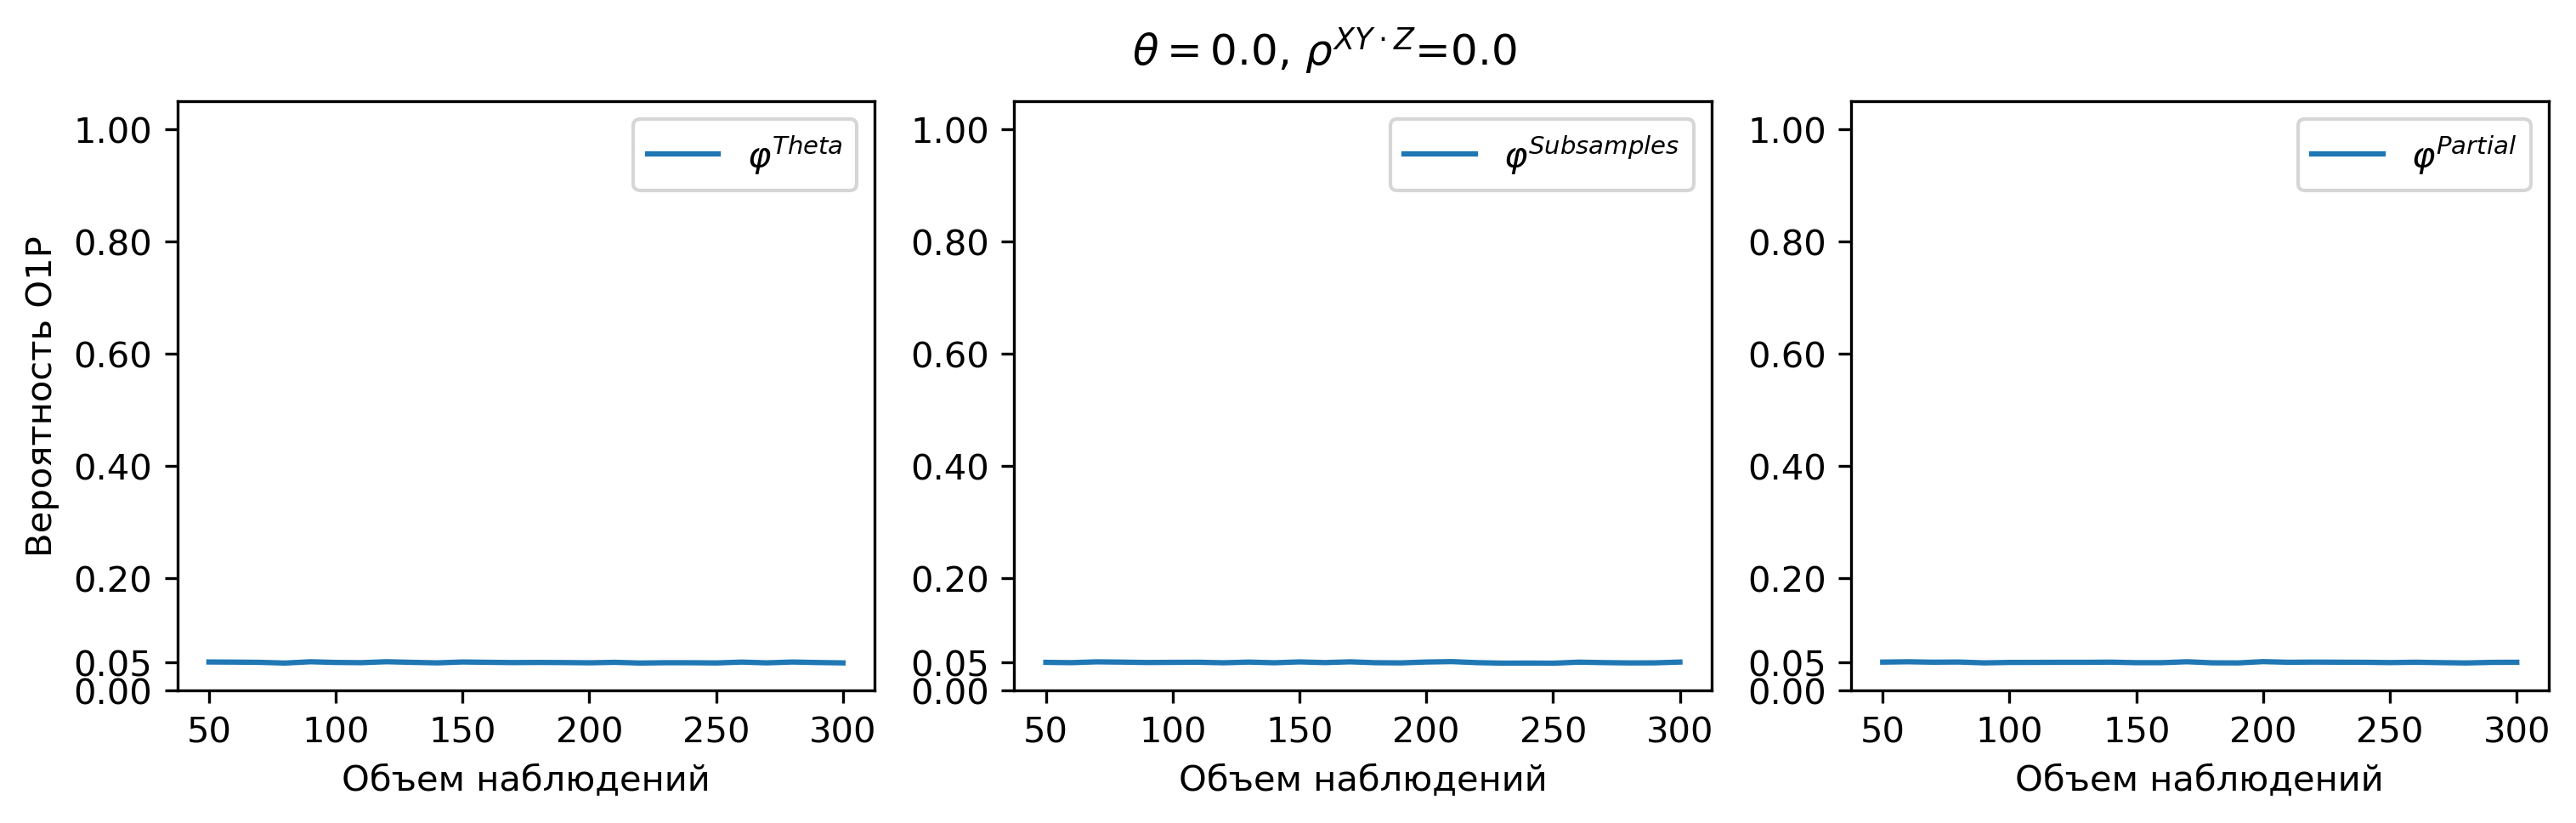
\includegraphics[scale=0.65]{images/graph1.png}
    \caption{Графики зависимости вероятности ошибки 1 рода (О1Р) от количества наблюдений,
     $p_{000}=0.125, p_{001}=0.125, p_{010}=0.125, p_{011}=0.125,
    p_{100}=0.125, p_{101}=0.125, p_{110}=0.125, p_{111}=0.125$. 
    Гипотезы $H: X \ci Y \mid Z$,
    $H^{\text{Theta}}: \theta=0$, 
    $H^{\text{Partial}}: \rho^{XY\cdot Z}~=~0$
    верны.
    Вероятность оценивается по $10^5$ экспериментам.} \label{fig:1}
\end{figure}
    

\begin{figure}[H]
    \centering
    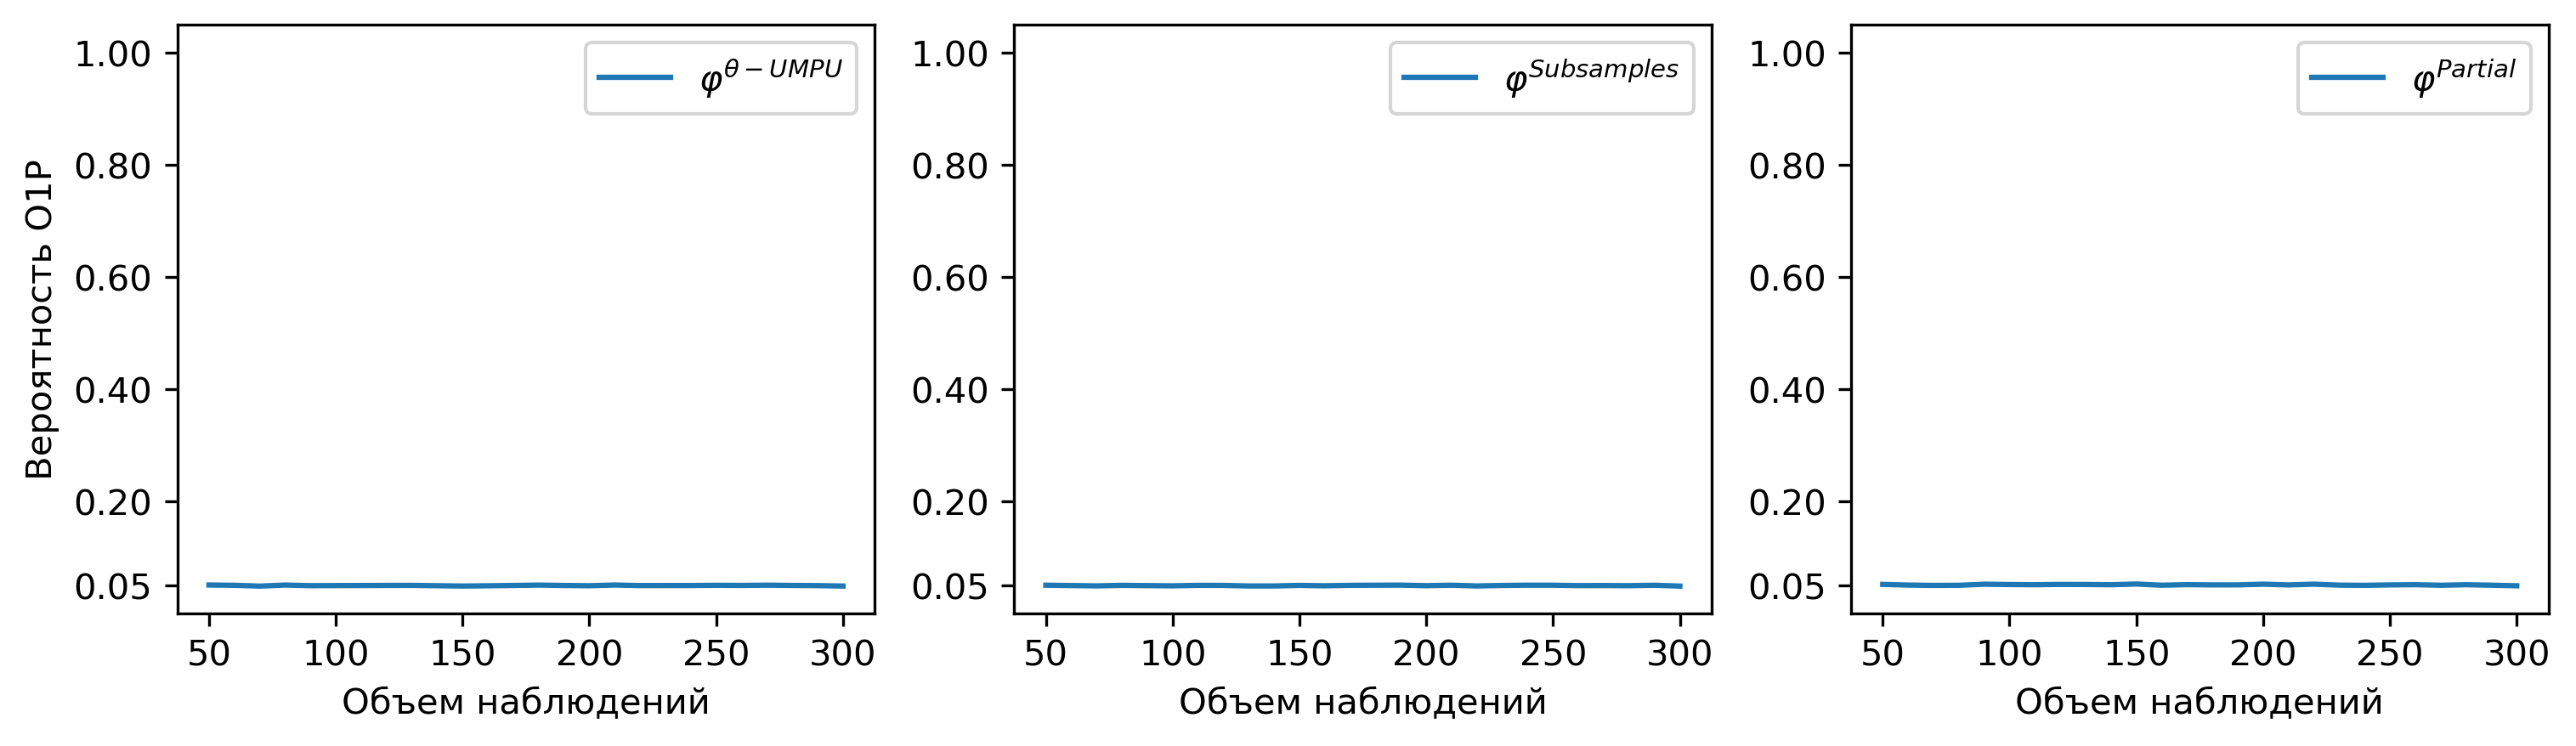
\includegraphics[scale=0.65]{images/graph2.png}
    \caption{Графики зависимости вероятности ошибки 1 рода (О1Р) от количества наблюдений,
    $p_{000}=0.15, p_{001}=0.1, p_{010}=0.3, p_{011}=0.1,
    p_{100}=0.05, p_{101}=0.1, p_{110}=0.1, p_{111}=0.1$. 
    Гипотезы $H: X \ci Y \mid Z$,
    $H^{\text{Theta}}: \theta=0$, 
    $H^{\text{Partial}}: \rho^{XY\cdot Z}=0$ верны.
    Вероятность оценивается по $10^5$ экспериментам.} \label{fig:2}
\end{figure}

\begin{figure}[H]
    \centering
    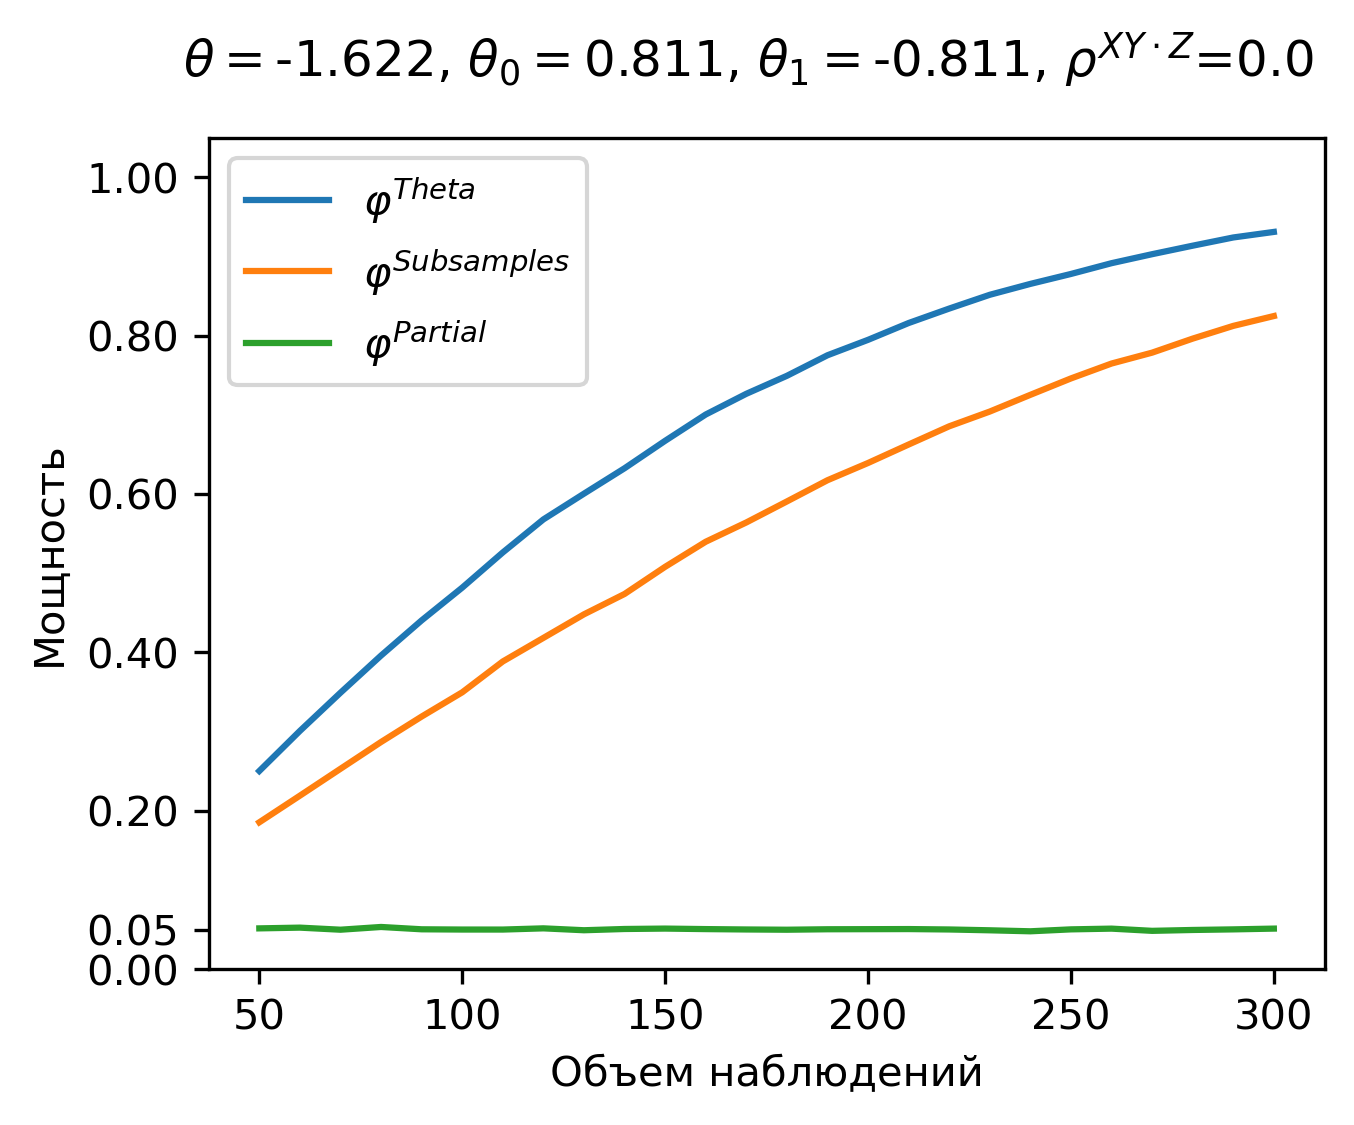
\includegraphics[scale=0.65]{images/graph4.png}
    \caption{График зависимости мощности от количества наблюдений,
    $p_{000}=0.15, p_{001}=0.1, 
    p_{010}=0.1, p_{011}=0.15,
    p_{100}=0.1, p_{101}=0.15, p_{110}=0.15, p_{111}=0.1$. 
    Гипотезы $H: X \ci Y \mid Z$,
    $H^{\text{Theta}}: \theta=0$ не верны.
    Гипотеза $H^{\text{Partial}}: \rho^{XY\cdot Z}=0$ верна.
    Мощность оценивается по $10^5$ экспериментам.} \label{fig:4}
\end{figure}

% Из (\autoref{fig:1}) и (\autoref{fig:2}) видно, что 
% для гипотезы $H: X \ci Y \mid Z$ тесты 
% $\varphi^{\text{Theta}}$, $\varphi^{\text{Subsamples}}$, контролируют вероятность 
% ошибки первого рода на уровне $\alpha=0.05$. Этот результат
% полностью согласуется с теорией из \autoref{expon_form_section}, 
% \autoref{twos}.

% (\autoref{fig:1}), (\autoref{fig:2}), (\autoref{fig:4}) показывают,
% что тест $\varphi^{\text{Partial}}$ контролирует вероятность
% ошибки первого рода на уровне $\alpha=0.05$ для гипотезы
% $H^\text{Partial}: \rho^{XY\cdot Z}=0$ в трехмерном
% распределении Бернулли. Этот результат является неожиданным,
% поскольку тест $\varphi^{\text{Partial}}$ теоретически обоснован
% лишь для трехмерного нормального распределения.
% Поскольку из $X \ci Y \mid Z$
% следует $\rho^{XY\cdot Z}=0$, то тест $\varphi^{\text{Partial}}$ также
% контролирует вероятность ошибки первого рода на уровне $\alpha=0.05$
% и для гипотезы $H: X \ci Y \mid Z$, что показано на 
% (\autoref{fig:1}), (\autoref{fig:2}).
% Однако, стоит отметить,
% что $\varphi^{\text{Partial}}$ проверяет необходимое условие 
% условной независимости. Поэтому может возникнуть ситуация
% как на (\autoref{fig:4}), когда гипотеза $H: X \ci Y \mid Z$ не верна, 
% но тест $\varphi^{\text{Partial}}$ не распознает отклонение от условной независимости, поскольку
% контролирует вероятность ошибки первого рода 
% на уровне $\alpha=0.05$ для гипотезы $H^{\text{Partial}}: \rho^{XY\cdot Z}=0$.

Из (\autoref{fig:1}) и (\autoref{fig:2}) видно, что тесты
$\varphi^{\text{Theta}}$ и $\varphi^{\text{Subsamples}}$ контролируют
вероятность ошибки первого рода 
на уровне
$\alpha=0.05$
для проверяемых гипотез 
$H: X \ci Y \mid Z$ и 
$H^{\text{Theta}}: \theta=0$ соответственно. Этот результат
полностью согласуется с теорией из \autoref{expon_form_section}, 
\autoref{twos}.

(\autoref{fig:1}), (\autoref{fig:2}), (\autoref{fig:4}) показывают,
что тест $\varphi^{\text{Partial}}$ контролирует вероятность
ошибки первого рода на уровне $\alpha=0.05$ для гипотезы\\
$H^\text{Partial}: \rho^{XY\cdot Z}=0$ 
в трехмерном
распределении Бернулли. Этот результат является неожиданным,
поскольку тест $\varphi^{\text{Partial}}$ теоретически обоснован
лишь для трехмерного нормального распределения.
Также стоит отметить, что на (\autoref{fig:1}), (\autoref{fig:2}), (\autoref{fig:4})
показаны ситуации, в которых верна гипотеза $H^\text{Partial}: \rho^{XY\cdot Z}=0$, но
гипотеза $H: X \ci Y \mid Z$ как верна (см.
(\autoref{fig:1}) и (\autoref{fig:2})), так и не верна 
(см. (\autoref{fig:4})). Поэтому принятие
гипотезы $H^\text{Partial}: \rho^{XY\cdot Z}=0$ не приводит
к выводам касательно истинности гипотезы $H: X \ci Y \mid Z$.

% \begin{figure}[H]
%     \centering
%     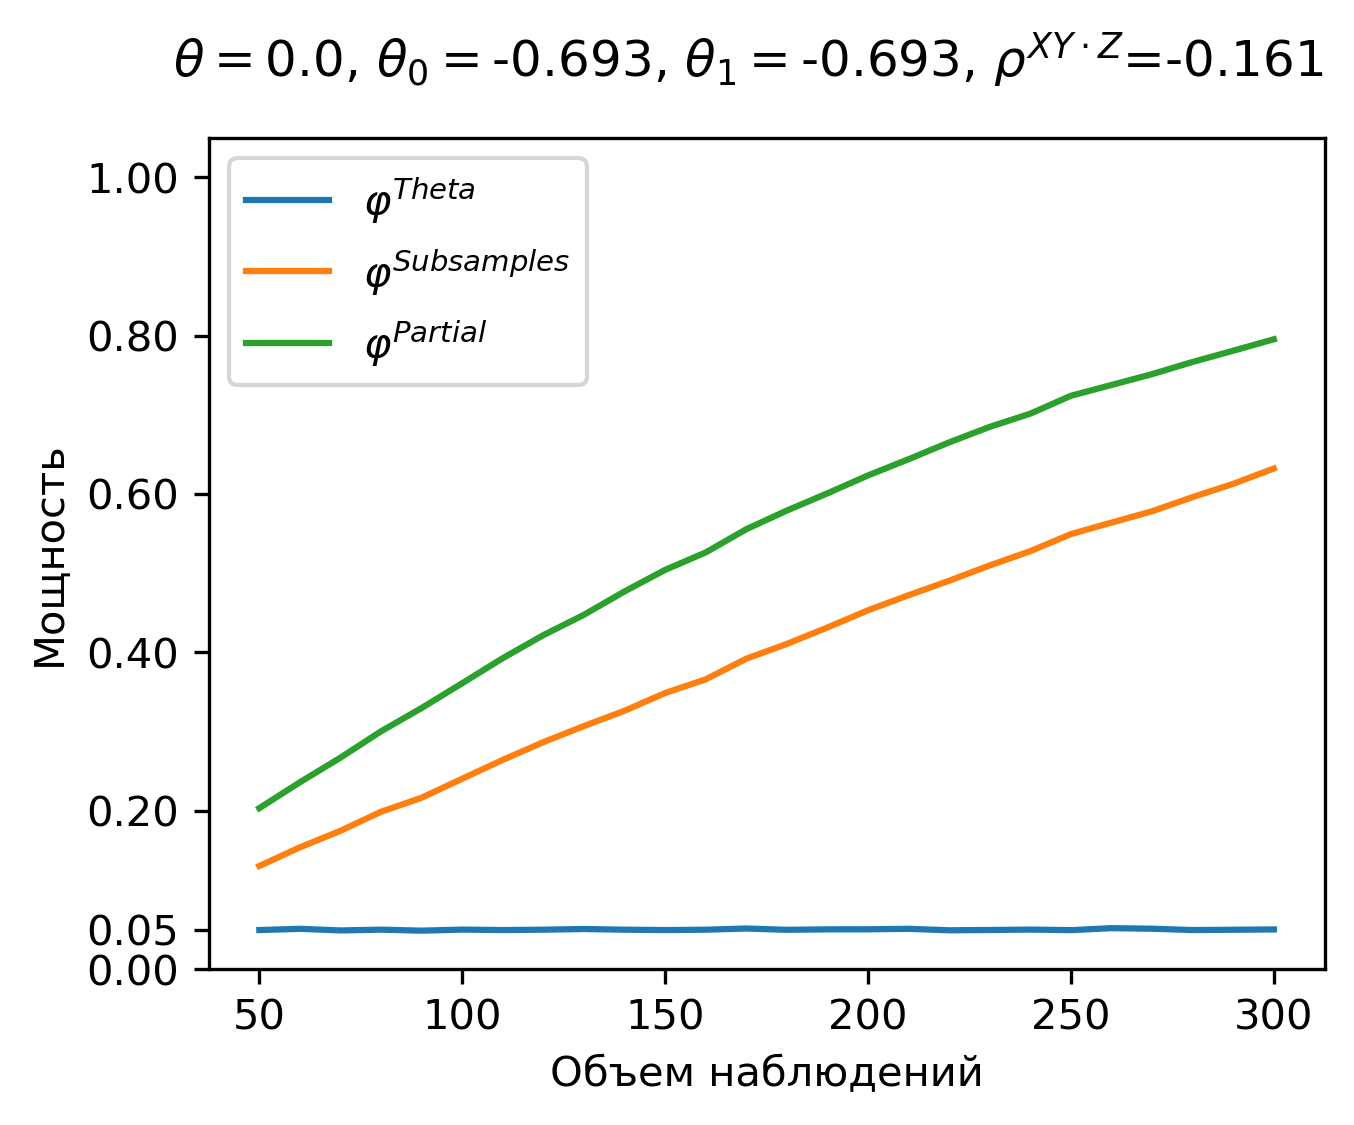
\includegraphics[scale=0.55]{images/graph5.png}
%     \caption{График зависимости мощности от количества наблюдений,
%     $p_{000}=0.15, p_{001}=0.05, 
%     p_{010}=0.3, p_{011}=0.1,
%     p_{100}=0.1, p_{101}=0.1, p_{110}=0.1, p_{111}=0.1$. 
%     Гипотеза $H: X \ci Y \mid Z$ не верна, однако верны гипотезы $H^{\text{Theta}}: \theta=0$
%     и $H^{\prime}: Y \ci Z \mid X$.
%     Мощность оценивается по $10^5$ экспериментам.} \label{fig:5}
% \end{figure}

% Напомним, что тест 
% $\varphi^{\text{Theta}}$ проверяет необходимое условие условной
% независимости. Так на (\autoref{fig:5}) гипотеза 
% $H: X \ci Y \mid Z$ не верна, 
% но тест $\varphi^{\text{Theta}}$
% не распознает отклонение от условной независимости и контролирует вероятность ошибки первого рода
% на уровне $\alpha=0.05$ для гипотезы $H^{\text{Theta}}: \theta=0$.

% Отметим, что $\varphi^{\text{Theta}}$ -- несмещенный тест уровня
% $\alpha$ проверки гипотезы $H: X \ci Y \mid Z$.
% Так как по \autoref{unbias} тест $\varphi^{\text{Subsamples}}$
% является несмещенным тестом уровня $\alpha$ проверки гипотезы $H: X \ci Y \mid Z$, и 
% на (\autoref{fig:5})
% тест $\varphi^{\text{Subsamples}}$ мощнее теста $\varphi^{\text{Theta}}$,
% то тест $\varphi^{\text{Theta}}$ не является РНМН тестом проверки 
% гипотезы $H: X \ci Y \mid Z$, хотя является РНМН тестом
% проверки гипотезы $H^{\text{Theta}}: \theta=0$.



\begin{figure}[H]
    \centering
    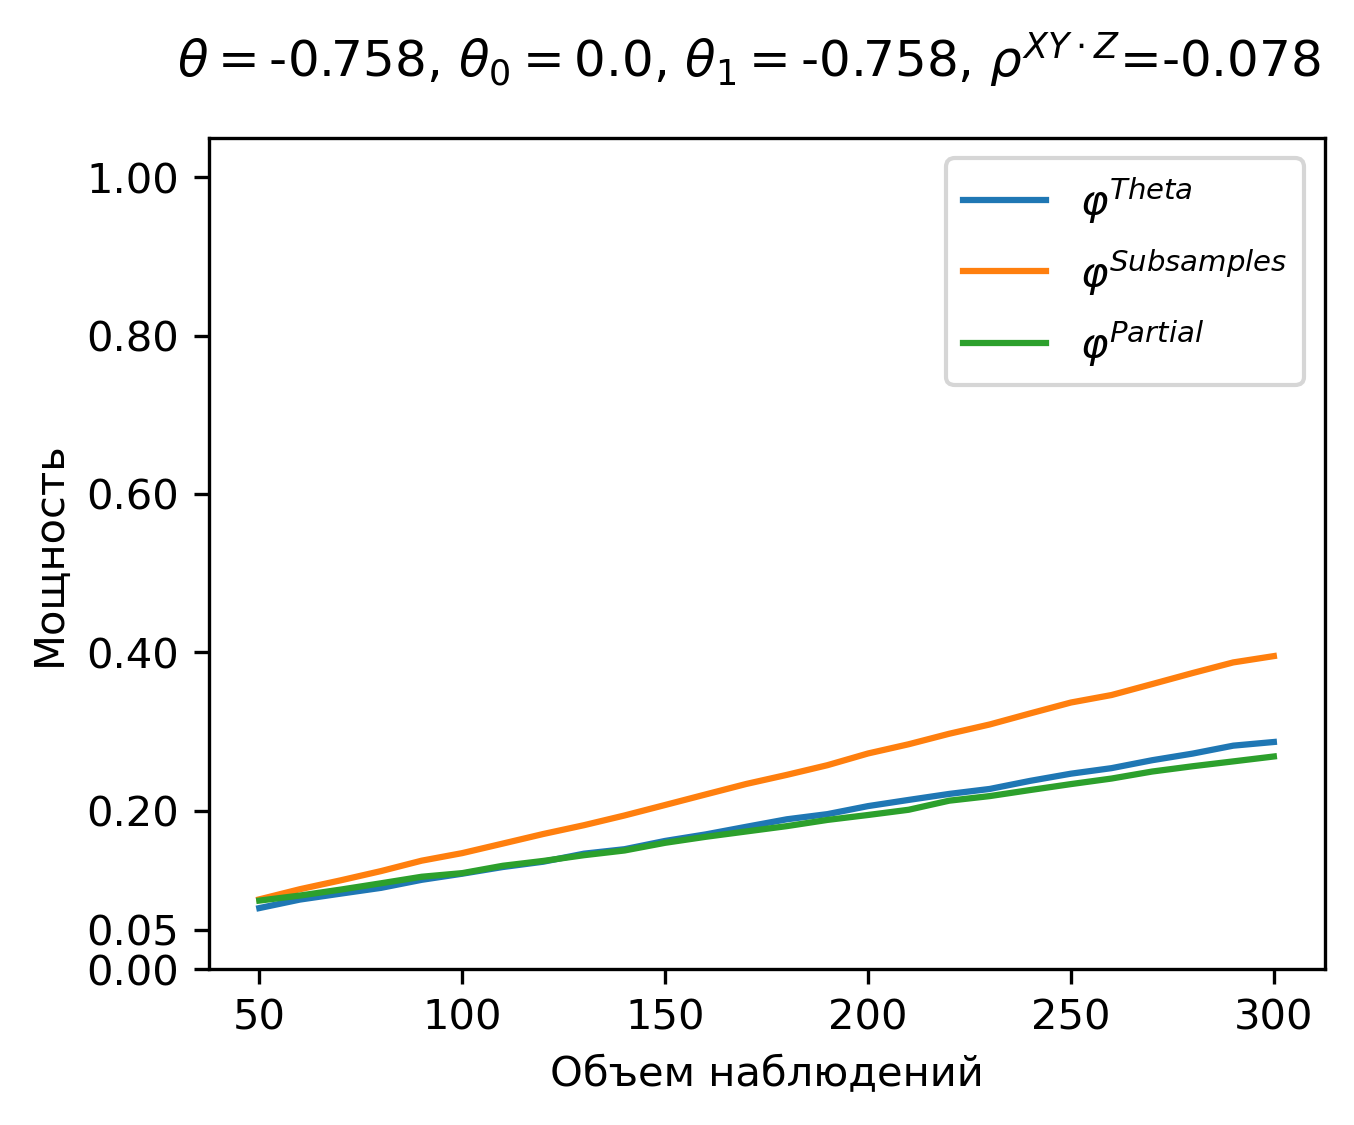
\includegraphics[scale=0.65]{images/graph3.png}
    \caption{График зависимости мощности от количества наблюдений,
    $p_{000}=0.15, p_{001}=0.06, 
    p_{010}=0.3, p_{011}=0.16,
    p_{100}=0.05, p_{101}=0.08, p_{110}=0.1, p_{111}=0.1$. 
    Гипотезы $H: X \ci Y \mid Z$,
    $H^{\text{Theta}}: \theta=0$, 
    $H^{\text{Partial}}: \rho^{XY\cdot Z}~=~0$
    не верны,
    однако $X$ и $Y$ независимы
    при условии $Z=0$. 
    Мощность оценивается по $10^5$ экспериментам.}\label{fig:3}
\end{figure}

\begin{figure}[H]
    \centering
    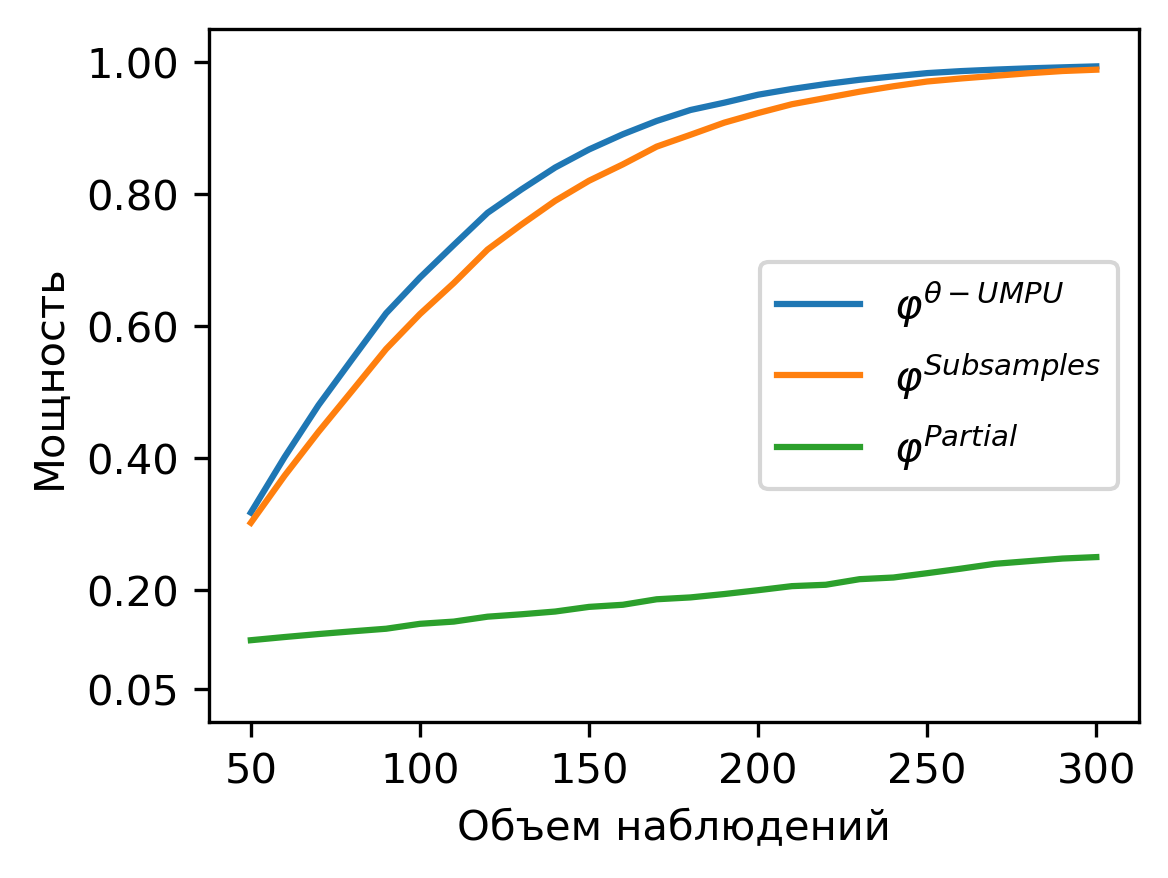
\includegraphics[scale=0.65]{images/graph6.png}
    \caption{График зависимости мощности от количества наблюдений,
    $p_{000}=0.03, p_{001}=0.1, 
    p_{010}=0.04, p_{011}=0.08,
    p_{100}=0.3, p_{101}=0.1, p_{110}=0.07, p_{111}=0.28$. 
    Гипотезы $H: X \ci Y \mid Z$,
    $H^{\text{Theta}}: \theta=0$, 
    $H^{\text{Partial}}: \rho^{XY\cdot Z}~=~0$
    не верны.
    Мощность оценивается по $10^5$ экспериментам.} \label{fig:6}
\end{figure}

\begin{figure}[H]
    \centering
    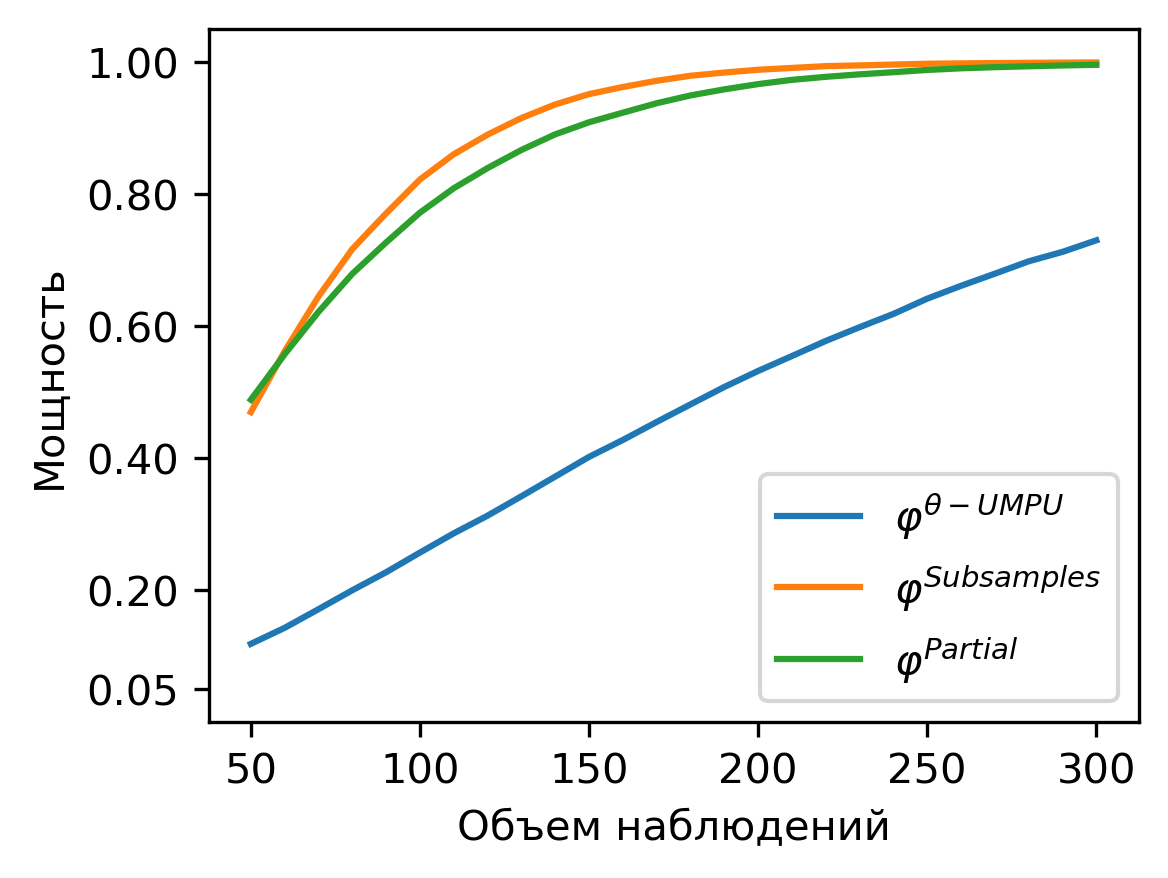
\includegraphics[scale=0.65]{images/graph7.png}
    \caption{График зависимости мощности от количества наблюдений,
    $p_{000}=0.21, p_{001}=0.12, 
    p_{010}=0.04, p_{011}=0.34,
    p_{100}=0.1, p_{101}=0.12, p_{110}=0.02, p_{111}=0.05$. 
    Гипотезы $H: X \ci Y \mid Z$,
    $H^{\text{Theta}}: \theta=0$, 
    $H^{\text{Partial}}: \rho^{XY\cdot Z}~=~0$
    не верны.
    Мощность оценивается по $10^5$ экспериментам.} \label{fig:7}
\end{figure}

Отвержение гипотез, проверяемых  тестами 
$\varphi^{\text{Theta}}$,
$\varphi^{\text{Subsamples}}$,
$\varphi^{\text{Partial}}$, влечет за собой решение о том, что
$X$ и $Y$ условно зависимы при условии $Z$.
(\autoref{fig:4}), 
(\autoref{fig:3}), (\autoref{fig:6}), (\autoref{fig:7})
показывают что при зависимости 
$X$ и $Y$ при условии $Z$ тест $\varphi^{\text{Subsamples}}$
оказывается мощнее теста $\varphi^{\text{Partial}}$.
(\autoref{fig:6}) показывает, что
мощность теста $\varphi^{\text{Partial}}$ зависит от истинного
значения частного коэффициента корреляции Пирсона. Кроме того, из (\autoref{fig:6})
видно, что при небольшом значении частного коэффициента корреляции
Пирсона тесты $\varphi^{\text{Theta}}$,
$\varphi^{\text{Subsamples}}$ демонстрируют высокую мощность.
Эти факты ставят под сомнение целесообразность использования 
на практике теста $\varphi^{\text{Partial}}$.

Стоит отметить, что при идентификации 0-1 графической модели
по наблюдениям
возникает необходимость множественной проверки гипотез\\
$H: X \ci Y \mid Z$, $H^{\prime}: X \ci Z \mid Y$, 
$H^{\prime \prime}: Y \ci Z \mid X$.
(\autoref{fig:4}) и (\autoref{fig:6}) показывают, что
в некоторых случаях тест $\varphi^{\text{Theta}}$, 
устанавливающий условную зависимость всех пар случайных величин,
оказывается мощнее теста $\varphi^{\text{Subsamples}}$, устанавливающего условную зависимость
одной пары случайных величин. 
Этот факт приводит к следующему способу идентификации графической
модели.
Сначала проверяется гипотеза
$H^{\text{Theta}}: \theta=0$. В случае её отвержения принимается
условная зависимость всех пар случайных величин. 
А в случае принятия гипотезы $H^{\text{Theta}}$ осуществляется 
дополнительная проверка гипотез $H$, $H^{\prime}$ и 
$H^{\prime \prime}$ тестом $\varphi^{\text{Subsamples}}$.


% (\autoref{fig:4}), (\autoref{fig:5}), 
% (\autoref{fig:3}), (\autoref{fig:6}), (\autoref{fig:7})
% показывают, что, вообще говоря, рассматриваемые тесты нельзя упорядочить по мощности.
% Кроме того, несмещенные тесты $\varphi^{\text{Subsamples}}$
% и $\varphi^{\text{Theta}}$ уровня $\alpha$ проверки
% гипотезы $H: X \ci Y \mid Z$ также нельзя упорядочить по мощности.
% Поэтому вопрос построения РНМН теста проверки гипотезы 
% $H: X \ci Y \mid Z$ остается открытым. 


% Одним из возможных отклонений от условной независимости является случай,
% когда $X$ и $Y$ независимы при условии $Z=0$, но зависимы при условии $Z=1$.
% Пример (\autoref{fig:3}) показывает, ...

% Показательным является пример с (\autoref{fig:6}). Тесты 
% $\varphi^{\text{Theta}}$ и $\varphi^{\text{Subsamples}}$ при $n=300$
% наблюдениях имеют мощность, близкую к $1$. В то время как мощность
% теста $\varphi^{\text{Partial}}$ приблизительно равна $0.25$. Это происходит потому, что
% в данном примере значение $\rho^{XY\cdot Z}=0.068$ близко к нулю.


% Еще интересен пример с (\autoref{fig:7}). 
% При $n=300$ наблюдениях мощность тестов
% $\varphi^{\text{Subsamples}}$, $\varphi^{\text{Partial}}$ близка к $1$,
% в то время как мощность теста $\varphi^{\text{Theta}}$ примерно равна $0.73$.

% В данном разделе были изложены результаты численных экспериментов с тестами
% $\varphi^{\text{Theta}}$, $\varphi^{\text{Subsamples}}$, 
% $\varphi^{\text{Partial}}$ при $\alpha=0.05$. На 
% (\autoref{fig:1}) и (\autoref{fig:2}) показано, что 
% при истинности гипотезы  
% $h: X \ci Y \mid Z$ эти тесты контролируют вероятность ошибки первого рода
% на уровне $\alpha=0.05$. 
% Однако, за счет того, что тесты 
% $\varphi^{\text{Subsamples}}$ и
% $\varphi^{\text{Partial}}$ проверяют более широкие гипотезы,
% возникают ситуации как на 
%  (\autoref{fig:4}) и (\autoref{fig:5}), когда гипотеза $h: X \ci Y \mid Z$
% не верна и мощность теста равна $0.05$ при любом объеме наблюдений.
% Особым образом можно выделить тест $\varphi^{\text{Subsamples}}$.
% На всех графиках $\varphi^{\text{Subsamples}}$ либо лучший по мощности,
% либо незначительно уступает лучшему по мощности тесту.
